In the following, SLIM is used in different configurations as a surrogate for modelling the benefit present values of two insurance tariffs. The results are interpreted and the fidelity is compared with the MBT algorithms GUIDE, MOB and CTree.

\subsection{Data set K2204}
The data set K2204 contains data for a (fictitious) endowment insurance tariff and includes the features sex (1 = male, 0 = female), age and duration and the two targets benefit present value (BPV) and premium present value (PPV). The targets were modelled using two different black box models.  
In the following, only the BPV is considered. The results for the PBV are very similar (interpreted the other way round) and can be found in the appendix.
Since the data set with 5994 observations is rather small, all observations were used for training. For this data set, we therefore only consider the training performance in the surrogate models.
A special characteristic of K2204 is a correlation between the features Age and Duration, as can be seen in Figure \ref{fig:ins_corr_age_duration}. When interpreting a MBT for this data set, it must therefore be taken into account that a split with regard to one of the features always has an influence on the value range of the other feature.

\begin{figure}[!htb]
    \centering    
    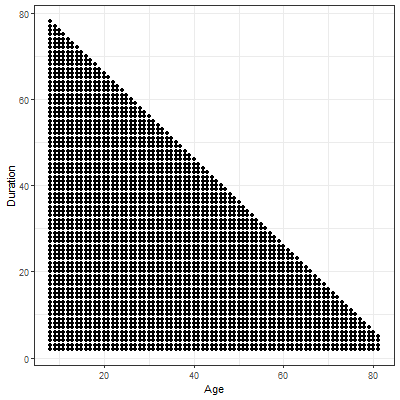
\includegraphics[width=7cm]{Figures/insurance_use_case/k2204_BPV/corr_age_duration.png}
    \caption{Features Age and Duration in the K2204 data set}
    \label{fig:ins_corr_age_duration}
\end{figure}


\subsubsection{Shallow MBTs with linear models}
In a first step, SLIM was fitted as surrogate to the black box predictions of BPV (BPV\_pred) with linear regression models in the nodes. The maximum depth was set to 3 and an improvement in the objective of at least 0.1 of the previous improvement was set as prepruning parameter.
 The resulting tree is shown in Figure \ref{fig:ins_slim_lm_tree}.

 \begin{figure}[!htb]
     \centering     
     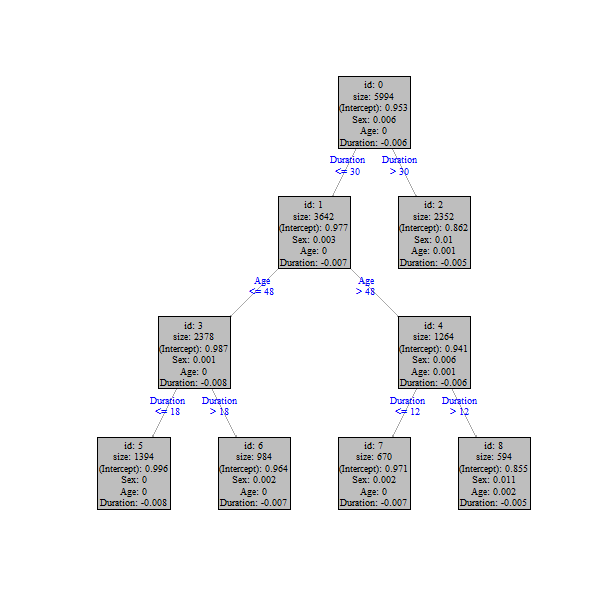
\includegraphics[width = 14cm]{Figures/insurance_use_case/k2204_BPV/slim_lm_tree.png}
     \caption{SLIM tree for K2204 with linear models}
     \label{fig:ins_slim_lm_tree}
 \end{figure}

Basic observations across all subregions are:
\begin{itemize}
    \item Gender male has a positive effect on BPV\_pred
    \item Age has a positive effect on BPV\_pred
    \item Duration has a negative effect on BPV\_pred
\end{itemize}

The strength of the effects, however, differs in the different subregions found by SLIM.
The five leafnodes can be roughly divided into two regions with similar effects:
\begin{itemize}
    \item Region 1 (Nodes 2,8): High Duration ($30$) or high Age ($>48$) and medium Duration (between $13$ and $30$)
    \item Region 2 (Nodes 5,6,7): Low - medium Duration with low Age or high Age with low Duration ($\leq 12$)
\end{itemize}

In Region 1 Sex male and Age have a higher positive effect on  BPV\_pred than in region 2. The negative effect of duration, on the other hand, is smaller in region 1. This indicates a non-linearity of duration.

If SLIM is fitted as a standalone model instead of a surrogate model in the same configuration, the differences in the split points are very small. This indicates that the black box model captures the underlying relationships very well. The corresponding tree is shown in the appendix in Figure \ref{fig:app_ins_slim_lm_standalone_tree}.

In the following, the fidelity of the different MBT with algorithms with linear models is compared. For this purpose, all four algorithms were fitted with a maximum depth of 3. For SLIM and GUIDE, impr is set to and for MOB and CTree alpha is set to 0.05. The MBTs are also compared with a baseline model, which is a linear model on the entire feature space. In addition to the $R^2$ and the MSE, the mean absolute error (MAE) and the maximum absolute error (max AE) were included as measures of fidelity. The max AEis particularly important here, as it is strictly regulated in order not to discriminate against any individual. 
The results are listed in table \ref{tab:ins_k2204_lm_surrogates_perf}. It shows that all MBTs achieve considerable improvement over the baseline model.

\begin{table}[!htb]

\caption{Performance of baseline linear model and MBTs with linear models}
\centering
\begin{tabular}[t]{l|r|r|r|r|r}
\hline
  & r2 & MSE & MAE & max AE & n leaves\\
\hline
lm & 0.985101 & 0.000201 & 0.011393 & 0.064709 & 1\\
\hline
SLIM & 0.999233 & 0.000010 & 0.002272 & 0.020526 & 8\\
GUIDE & 0.999276 & 0.000010 & 0.002142 & 0.020526 & 8\\
MOB & 0.998527 & 0.000020 & 0.003149 & 0.024504 & 8\\
CTree & 0.995091 & 0.000066 & 0.005740 & 0.042931 & 8\\
\hline
\end{tabular}
\label{tab:ins_k2204_lm_surrogates_perf}
\end{table}

GUIDE achieves the best performance slightly ahead of SLIM. Ctree's performance is considerable behind the other algorithms.
Since all algorithms generate MBTs with the same number of leafnodes, the difference in performance must be explained by different split points.
Table \ref{tab:ins_k2204_lm_surrogates_share} lists the share of observations that were split with respect to the different features.

\begin{table}[!htb]

\caption{Share of observations split by the different features}
\centering
\begin{tabular}[t]{l|r|r|r}
\hline
& Age & Duration & Sex\\
\hline
SLIM & 0.28 & 0.67 & 0.05\\
GUIDE & 0.28 & 0.72 & 0.00\\
MOB & 0.10 & 0.77 & 0.13\\
CTree & 0.00 & 0.96 & 0.04\\
\hline
\end{tabular}
\label{tab:ins_k2204_lm_surrogates_share}
\end{table}

It is noticeable that SLIM and GUIDE split by age more often than the other two algorithms.

\subsubsection{Shallow MBTs with B-spline models}

In order to better capture non-linearities and thus reduce the risk of splitting with respect to non-linearities instead of interactions, all MBT algorithms are then fitted with B-spline transformed feature age and duration as surrogate models. The max depth is again set to 3 in order to obtain interpretable shallow trees. Again, a baseline was fitted, in this case a regression model with B-spline transformed features Age and Duration on the entire feature space. The fidelity results are listed in table \ref{tab:ins_k2204_bsplines_small_surrogates_perf}.

\begin{table}

\caption{Performance of baseline model and MBTs with B-spline transformations}
\centering
\begin{tabular}[t]{l|r|r|r|r|r}
\hline
  & $R^2$ & MSE & MAE & max AE & n leaves\\
\hline
lm bsplines & 0.9943311 & 7.63e-05 & 0.0067811 & 0.0378568 & 1\\
\hline
SLIM & 0.9994176 & 7.80e-06 & 0.0018244 & 0.0167730 & 8\\
GUIDE & 0.9993900 & 8.20e-06 & 0.0019011 & 0.0165545 & 8\\
MOB & 0.9992115 & 1.06e-05 & 0.0022236 & 0.0182034 & 8\\
CTree & 0.9990918 & 1.22e-05 & 0.0024194 & 0.0183906 & 8\\
\hline
\end{tabular}
\label{tab:ins_k2204_bsplines_small_surrogates_perf}
\end{table}

The improvement over the baseline model is also large here, but not as substantial as in the trees with linear models without B-spline transformations. This is probably due to the fact that the splits in the MBTs with linear models also handled non-linearities that could not be adjusted in the linear baseline model. In the baseline model with bspline transformations, on the other hand, the non-linearities are already taken into account and the splits then actually capture primarily the interactions, which is what is desired. 


Table \ref{tab:ins_k2204_bsplines_small_surrogates_share}  shows the proportions of observations that were split according to the different features. 


\begin{table}[!htb]
\caption{Share of observations split by the different features}
\centering
\begin{tabular}[t]{l|r|r|r}
\hline
  & Age & Duration & Sex\\
\hline
SLIM & 0.38 & 0.62 & 0.00\\
GUIDE & 0.30 & 0.70 & 0.00\\
MOB & 0.08 & 0.84 & 0.08\\
CTree & 0.23 & 0.71 & 0.07\\
\hline
\end{tabular}
\label{tab:ins_k2204_bsplines_small_surrogates_share}
\end{table}

For SLIM, GUIDE and MOB these results are similar to the MBTs with linear models. CTree, on the other hand, now also selects Age in $23\%$ of split observations as splitting variable, whereas it was not used at all for splitting in CTree with linear models. CTree performs the worst in terms of fidelity in this case as well, but not as considerable as in the previous setting.
For the interpretation, we will again take a closer look at the SLIM tree

\begin{figure}[!htb]
    \centering   
    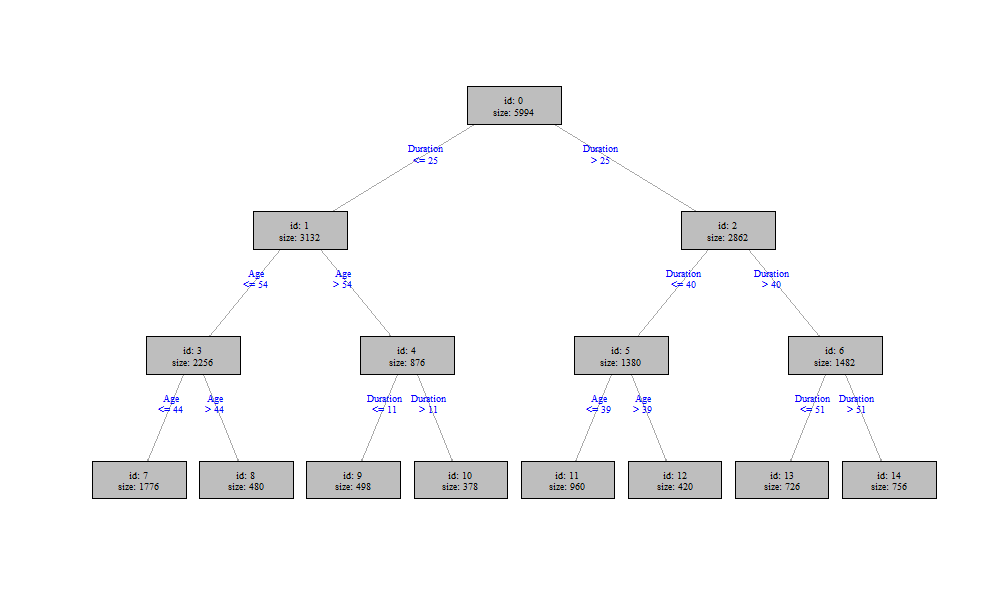
\includegraphics[width = 16cm]{Figures/insurance_use_case/k2204_BPV/slim_bsplines_small_tree.png}
         \caption{SLIM tree for K2204 with B-spline models}
     \label{fig:ins_slim_bsplines_tree}
\end{figure}

In order to investigate the effects of the splits on the feature effects more closely, the splits with regard to duration and age are analysed separately.
The nodes 1,5,13 and 14 together comprise the entire feature space, whereby the sub-regions are determined by splits with regard to the feature duration.
Figure \ref{fig:ins_k2204_effects_duration} shows the input-output relation (feature effects) of the features estimated in the B-spline models in the different nodes. Note that the effects are centred.

\begin{figure}[!htb]
    \centering
    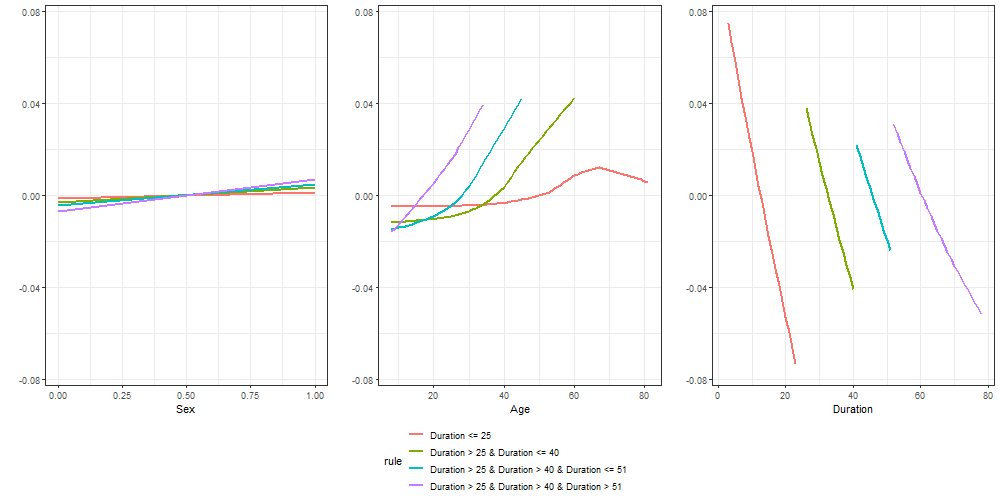
\includegraphics[width = 16cm]{Figures/insurance_use_case/k2204_BPV/effects_duration.png}
    \caption{Input-output relation of features in nodes split by duration for SLIM tree with B-splines and depth 3}
    \label{fig:ins_k2204_effects_duration}
\end{figure}

As with SLIM with linear models, it can be seen that the positive effect of male gender increases with increasing duration. The same applies to Age. The seemingly negative effect of age at low maturity and high age is probably due to extrapolation. There are only a few observations in this area, as can be seen in Figure \ref{fig:ins_k2204_hist_age}.

\begin{figure}[!htb]
    \centering
    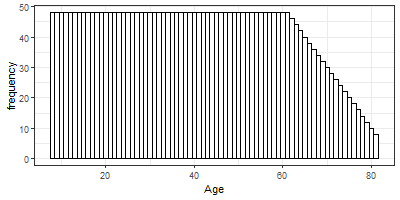
\includegraphics[width = 14cm]{Figures/insurance_use_case/k2204_BPV/hist_age.png}
    \caption{Frequency of observations with respect to feature Age}
    \label{fig:ins_k2204_hist_age}
\end{figure}


\subsection{Data set R1\_08}



